%% Le lingue utilizzate, che verranno passate come opzioni al pacchetto babel. Come sempre, l'ultima indicata sar� quella primaria.
%% Se si utilizzano una o pi� lingue diverse da "italian" o "english", leggere le istruzioni in fondo.
\def\thudbabelopt{english}
%% Valori ammessi per target: bach (tesi triennale), mst (tesi magistrale), phd (tesi di dottorato).
%% Valori ammessi per aauheader: '' (vuoto -> nessun header Alpen Adria Univeristat), aics (Department of Artificial Intelligence and Cybersecurity), informatics (Department of Informatics Systems). Il nome del dipartimento � allineato con la versione inglese del logo UniUD.
\documentclass[target=bach,aauheader=]{thud}

%% --- Informazioni sulla tesi ---
%% Per tutti i tipi di tesi
% Scommentare quello di interesse, o mettete quello che vi pare
\course{Internet of Things, Big Data and Web}
\title{Comparison of tools for the formal verification of MTProto 2.0}
\author{Alessandro Zanatta}
\supervisor{Prof.\ Marino Miculan}
%% Campi obbligatori: \title, \author e \course.
%% Altri campi disponibili: \reviewer, \tutor, \chair, \date (anno accademico, calcolato in automatico), \rights
%% Con \supervisor, \cosupervisor, \reviewer e \tutor si possono indicare pi� nomi separati da \and.

%% --- Pacchetti consigliati ---
%% pdfx: per generare il PDF/A per l'archiviazione. Necessario solo per la versione finale
\usepackage[a-1b]{pdfx}
%% hyperref: Regola le impostazioni della creazione del PDF... pi� tante altre cose. Ricordarsi di usare l'opzione pdfa.
\usepackage[pdfa]{hyperref}
%% tocbibind: Inserisce nell'indice anche la lista delle figure, la bibliografia, ecc.

%% --- Stili di pagina disponibili (comando \pagestyle) ---
%% sfbig (predefinito): Apertura delle parti e dei capitoli col numero grande; titoli delle parti e dei capitoli e intestazioni di pagina in sans serif.
%% big: Come "sfbig", solo serif.
%% plain: Apertura delle parti e dei capitoli tradizionali di LaTeX; intestazioni di pagina come "big".

%% --- Other packages --- %%
% Protocol graphical representation
\usepackage{msc}
\usepackage{mathtools}
\usepackage{amssymb}


%% --- Commands --- %%
\newcommand\setmscoptions{%
  \setlength{\instdist}{5cm}%
  % \setlength{\levelheight}{1.5 \levelheight}%
  % \setlength{\instwidth}{3cm}
  \setmsckeyword{}
  \drawframe{no}
  \centering
}

\newcommand*{\Z}{\mathbb{Z}}

%% --- Document start --- %%
\begin{document}
\maketitle

%% Dedica (opzionale)
\begin{dedication}
	Al mio cane,\par per avermi ascoltato mentre ripassavo le lezioni.
\end{dedication}

%% Ringraziamenti (opzionali)
\acknowledgements
Ringraziamenti vari qua

%% Sommario (opzionale)
\abstract
Un bell'abstract va qua!

%% Indice
\tableofcontents

%% Lista delle tabelle (se presenti)
%\listoftables

%% Lista delle figure (se presenti)
%\listoffigures

%% Corpo principale del documento
\mainmatter

%% Parte
%% La suddivisione in parti � opzionale; solitamente sono sufficienti i capitoli.
%\part{Parte}

%% Capitolo
\chapter{Introduction}


\chapter{Proverif and Tamarin}


\chapter{MTProto2.0 protocol description}

In this chapter, we will give a brief overview of the MTProto2.0 protocol. A more in-depth and formal description can be found on the official web page \cite{Telegram-MTProto2.0}.

First of all, MTProto2.0 is a \textit{suite of protocols} used to enable secure communication between a Telegram client and a Telegram server over an insecure network. MTProto2.0 can be decomposed in the three following protocols:

\begin{description}[style=nextline]
    \item[Authorization] used to obtain a secret authorization key shared only with the server;
    \item[Secret-chat] used to obtain a secret key shared between two clients. This is then used to exchange end-to-end messages between two clients, with the server that basically acts as a forwarder;
    \item[Rekeying] used to achieve Perfect Forward Secrecy, allows obtaining a new end-to-end encryption key.
\end{description}

Additionally, the cloud chats encryption schema is used to securely exchange messages between clients and servers (who have shared an authorization key).

An overview on these protocols will be given in \cref{sec:auth-prot,sec:cloud-chat,sec:secret-chat,sec:rekeying}.

\section{Authorization protocol}
\label{sec:auth-prot}

%% Authorization protocol %%
\begin{figure}[!t]
\setlength{\instdist}{4cm}
\setmscoptions
\begin{msc}{}
\setmscscale{.8} 

\declinst{client}{}{Client}
\declinst{server}{}{Server}

\action*{Generates nonces $n_{c}, n_{k}$}{client}
\action*{\parbox{4.5cm}{\centering 
    Knows keys $\mbox{sk}^{(1)}, \dots, \mbox{sk}^{(n)}$\\
    Generates $n_s, g, p$\\
    Generates proof-of-work primes $q, r$
}}{server}
\nextlevel[6]

\mess{$n_{c}$}{client}{server}
\nextlevel[2]
\mess{$n_{c}, n_{s}, q \cdot r, \mbox{fp}^{(1)}, \dots, \mbox{fp}^{(n)}$}{server}{client}

\nextlevel
\action*{\parbox{4cm}{\centering
    Chooses $\mbox{pk}^{(i)}$ matching\\
    $\mbox{fp}^{(i)}$ for some $i$\\
    Factorizes $q \cdot r$\\
    $C_1 := q \cdot r, q, r, n_c, n_s, n_k$
}}{client}

\nextlevel[7]
\mess{$n_c, n_s, q, r, \mbox{fp}^{(i)}, \{\mbox{sha1}\left(C_1\right), C_1\}_{\mbox{pk}^{(i)}}$}{client}{server}
\nextlevel

\action*{$\left(k, iv\right) := \mbox{kdf}\left(n_s, n_k\right)$}{client}
\action*{\parbox{4.5cm}{\centering
    $s \in \Z_p$\\
    $g_s := g^s \mod{p}$\\
    $key, iv := \mbox{kdf}\left(n_s, n_k\right)$\\
    $S_1 := n_c, n_s, g, p, g_s, t_1$
}}{server}

\nextlevel[6]
\mess{$n_c, n_s, \left\{\mbox{sha1}\left(S_1\right), S_1\right\}_{key, iv}$}{server}{client}
\nextlevel

\action*{\parbox{4.5cm}{\centering
$c \in \Z_p$\\
$g_c := g^c \mod{p}$\\
Checks $g, p$\\
$k_{CS} := g_s^c \mod{p}$\\
$C_2 := n_c, n_s, rID, g_c$
}}{client}
\nextlevel[7]

\mess{$n_c, n_s, \left\{\mbox{sha1}\left(C_2\right), C_2\right\}_{k, iv}$}{client}{server}
\nextlevel

\action*{\parbox{4.5cm}{\centering
$k_{CS} := g_c^s \mod{p}$
}}{server}
\nextlevel[3]

\mess{$n_c, n_s, \mbox{hash}\left(n_k, k_{CS}\right)$}{server}{client}


\end{msc}
\centering
\caption{MTProto2.0 Authorization protocol}
\label{fig:authorization-protocol}
\end{figure}


The first time a Telegram client C runs the application, it must negotiate an \textbf{authorization key} with the Telegram server S. The authorization protocol is used to this end. Once the client and the server have shared an authorization key, they will use it to encrypt (almost) every future communication between them. A client might also have several keys (e.g. on multiple devices or if reinstalling the application), some of which might be locked (e.g. if the device is lost). The authorization protocol is based on the Diffie-Hellman key exchange protocol \cite{DH-protocol}.


A successful protocol run consists of three rounds, which are represented schematically in \cref{fig:authorization-protocol}:
\begin{description}
    \item[Round 1] In the first round messages are in plaintext. In particular, the client and the server exchange two nonces ($n_c$ and $n_s$). The pair $\left<n_c, n_s\right>$ identifies a session of the authorization protocol. These nonces are sent in every consequent message of the current run of the protocol, both in plaintext and encrypted form.
    \begin{enumerate}
        \item{In the first message, the client sends his fresh nonce $n_c$ to the server;}
        \item{The server answers with the client nonce $n_c$, the server fresh nonce $n_s$, a challenge $q \cdot r \leq 2^{63}$ (which are two primes used as a measure to prevent denial of service, as the client needs to spend resources on factorizing $q \cdot r$ before the server has to commit (more) resources\footnote{Notice that this might not be true as this is vulnerable to a lookup table approach (e.g. using \href{http://factordb.com}{factordb.com}).}) and a list of public RSA key fingerprints (calculated as the lower 64-bits of the SHA1 of the server public keys).}
    \end{enumerate}

    \item[Round 2] The client decomposes $q\cdot r$ in $\left<q, r\right>$, retrieves the public key of the server $pk^{\left(i\right)}$. The client then generates a nonce $n_k$ of 256 bits. This nonce $n_k$ is supposed to be secret. The pair $\left<n_s, n_k\right>$ is used, by both server and client, to derive, through a derivation function $\mbox{kdf}$, a symmetric encryption key $k$ and an initialization vector $iv$, which will be used in subsequent exchanges.
    \begin{enumerate}
        \setcounter{enumi}{2}
        \item{The client asymmetrically encrypts both $\left<q\cdot r, q, r, n_c, n_s, n_k\right>$ and its SHA1 hash with $pk^{(i)}$ and sends it along with $\left<n_c, n_s, q, r, fp^{(i)}\right>$ to the server. A rather complex padding schema is used;}
        \item{The server generates his Diffie-Hellman ephemeral key $s$ of 2048-bits, chooses $g, p$ and computes $g_s = g^s \mod{p}$. Finally, it symmetrically encrypts both $\left<n_c, n_s, g, p, g_s, t_1\right>$ and its SHA1 hash and sends it along with $\left<n_c, n_s\right>$.}
    \end{enumerate}

    Notice that the client is supposed to check that:
    \begin{itemize}
        \item{$p$ is a safe 2048-bit prime, where safe means that both $p$ and $\frac{p-1}{2}$ are prime and $2^{2047} < p < 2^{2048}$;}
        \item{$g$ is a generator for $\frac{p-1}{2}$.}
    \end{itemize}

    \item[Round 3] In the last round, the client generates his own Diffie-Hellman ephemeral key and shares it with the server.
    \begin{enumerate}
        \setcounter{enumi}{4}
        \item{The client generates his ephemeral key $c$ of 2048-bits and computes $g_c = g^c \mod{p}$. Then, it symmetrically encrypts both $\left<n_s, n_s, retryID, g_c\right>$ and its SHA1 hash and sends them along with $\left<n_c, n_s\right>$. The $retryID$ starts at zero at the time of the first attempt, otherwise is based on the values from the last failed attempt;}
        \item{The server is now able to compute the authorization key as $k_{CS} = g_c ^ s \mod{p}$. Assuming server checks pass, S sends an acknowledgment for the new key: $\left<n_c, n_s, \mbox{hash}\left(k_{CS}\right)\right>$.}
    \end{enumerate}

\end{description}

\subsection{Implementation notes}
TODO (?)








\section{Cloud-chat encryption schema}
\label{sec:cloud-chat}

%% Cloud-chat encryption schema %%
\begin{figure}[t]
    \centering
    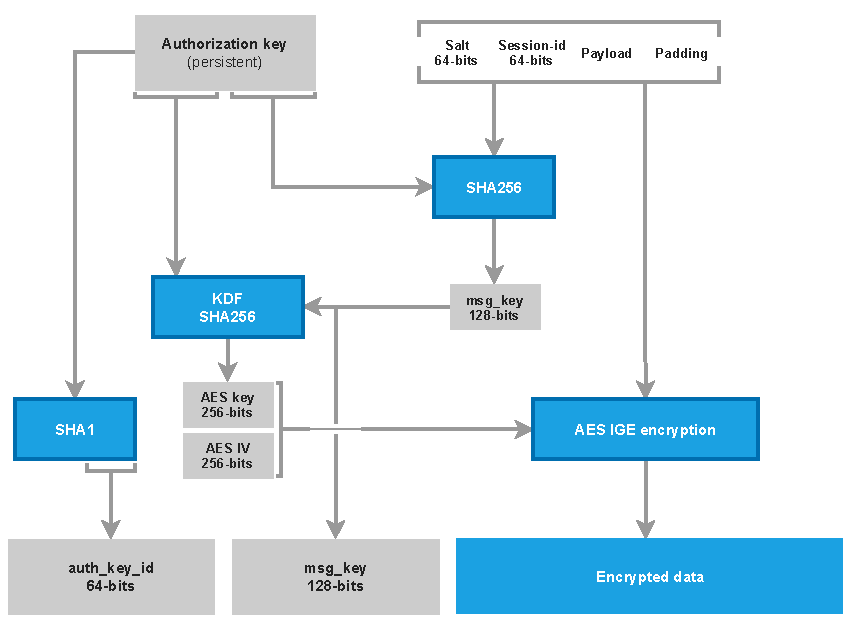
\includegraphics{cloud-chats}
    \caption{MTProto2.0 Cloud-chat protocol.\\Representation inspired by the Telegram official one.}
    \label{fig:cloud-chat-protocol}
    \end{figure}

Telegram uses the schema in \cref{fig:cloud-chat-protocol} to encrypt every message exchanged between the client and the server after an authorization key has been established using the authorization protocol in \cref{sec:auth-prot}.

A message key \textbf{msg\_key} of 128 bits is calculated as the middle 128 bits of the SHA256 of the entire message prepended by 32 bytes of the authorization key. The message itself contains a 64-bit salt, a 64-bit session id, the payload\footnote{The payload contains the time of the message, its length, a sequence number. Receiver should check these pieces of information, after decryption.} and a variable size padding of 12-1024 bytes.
The authorization key \textbf{auth\_key}, combined with the message key \textbf{msg\_key}, is used to derive a key and an initialization vector, which are used to encrypt the entire message using AES in IGE mode.

\subsection{IGE mode}
Infinite Garble Extension (in short, IGE) is a block cipher mode, lesser-known than others like ECB, CBC, OFB, CTR, CFB, GCM, CCM.
IGE can be defined with the following formula:

\begin{equation}
c_i = f_K(m_i \oplus c_{i-1}) \oplus m_{i-1}
\end{equation}

where $f_K$ stands for the encrypting function (like AES) with key $K$
and $i$ goes from 1 to $n$ $–$ the number of plaintext blocks. Two initialization vectors are also needed. \Cref{fig:IGE} summarizes how the encryption in IGE mode works.

\begin{figure}[t]
    \centering
    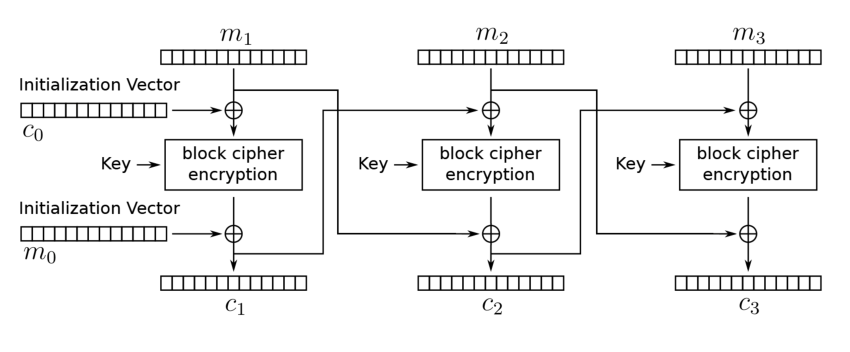
\includegraphics{IGE}
    \caption{Encryption in IGE mode.}
    \label{fig:IGE}
\end{figure}

One of the main properties of IGE mode is that it makes sure that if a ciphertext block is changed, then every subsequent block following it will not decrypt correctly.

As pointed out by \cite{Telegram-AFAQ-IGE}, the Telegram developers team is aware of the vulnerability of this mode to blockwise-adaptive Chosen Plaintext Attack (CPA)\cite{IGE-CPA}, but they claim that MTProto is not affected.




\section{Secret-chat protocol}
\label{sec:secret-chat}

%% Secret-chat protocol %%
\begin{figure}[!t]
\setlength{\instdist}{3cm}
\setmscoptions
\begin{msc}{}
\setmscscale{.8} 

\declinst{alice}{}{Alice}
\declinst{server}{}{Server}
\declinst{bob}{}{Bob}


\action*{\parbox{4.5cm}{\centering
    Knows $k_{AS}, k_{BS}$
}}{server}

\action*{\parbox{4.5cm}{\centering
    Knows $k_{AS}$
}}{alice}

\action*{\parbox{4.5cm}{\centering
    Knows $k_{BS}$
}}{bob}

\nextlevel[2]
\action*{\parbox{4.5cm}{\centering
    Gets $g, p$\\
    Generates $sid$\\
    $a \in \Z_p$\\
    $g_a := g^a \mod{p}$\\
    $M_1 := g, p, sid, g_a$
}}{alice}

\nextlevel[7]

%% TODO: Telegram webpage does not seem to specify HOW this is encrypted!!
%% UPDATE: It actually (kinda) does: it's encrypted as a cloud-chat message! For simplicity, keep this notation and explain its meaning in the written part.
\mess{$\left\{M_1\right\}_{k_{AS}}$}{alice}{server}
\nextlevel
\mess{$\left\{M_1\right\}_{k_{BS}}$}{server}{bob}

\nextlevel
\action*{\parbox{4.5cm}{\centering
    $b \in \Z_p$\\
    $g_b := g^b \mod{p}$\\
    $k_{AB} := g_a ^ b \mod{p}$\\
    $M_2 := sid, g_b, \mbox{fpk}\left(k_{AB}\right)$
}}{bob}

\nextlevel[6]
\mess{$\left\{M_2\right\}_{k_{BS}}$}{bob}{server}
\nextlevel
\mess{$\left\{M_2\right\}_{k_{AS}}$}{server}{alice}

\nextlevel
\action*{\parbox{5cm}{\centering
    $k_{AB} := g_b ^ a \mod{p}$\\
    Generates $payload$\\
    $mk := \mbox{sha256}\left(k_{AB}, payload\right)$\\
    $key, iv = \mbox{kdf}\left(k_{AB}, mk\right)$\\
    $C := \left\{payload\right\}_{key, iv}$
    $msg := \mbox{fpk}\left(k_{AB}\right), mk, C$
}}{alice}

\nextlevel[8]
\mess{$\left\{msg\right\}_{k_{AS}}$}{alice}{server}
\nextlevel
\mess{$\left\{msg\right\}_{k_{BS}}$}{server}{bob}

\end{msc}

\centering
\caption{MTProto2.0 Secret-chat protocol}
\label{fig:secret-chat-protocol}
\end{figure}

Telegram secret chats deal with end-to-end encryption between two clients (as usual, let us call the clients Alice and Bob, or A and B for brevity). After both clients have shared an authorization key with the Telegram server S, they can decide to engage themselves in a run of the secret chat protocol, allowing them to share, using a Diffie-Hellman key exchange, a shared secret. Notice that the server acts as a forwarder: every message sent from a client A to another client B is sent to the server, encrypted as a cloud chat message shown in \cref{sec:cloud-chat} with the authorization key of A; the server then decrypts the message and encrypts it as a cloud chat message using the authorization key of B and finally sends it to B. The writing $\left\{M\right\}_{k_{AS}}$ in \cref{fig:secret-chat-protocol} expresses that the message $M$ has been encrypted with the authorization key $k_{AS}$ using the cloud chat encryption schema.




\section{Rekeying protocol}
\label{sec:rekeying}


%% Fine dei capitoli normali, inizio dei capitoli-appendice (opzionali)
\appendix

%\part{Appendici}

\chapter{Titolo della prima appendice}

%% Parte conclusiva del documento; tipicamente per riassunto, bibliografia e/o indice analitico.
\backmatter

%% Riassunto (opzionale)
%\summary
%Maecenas tempor elit sed arcu commodo, dapibus sagittis leo egestas. Praesent at ultrices urna. Integer et nibh in augue mollis facilisis sit amet eget magna. Fusce at porttitor sapien. Phasellus imperdiet, felis et molestie vulputate, mauris sapien tincidunt justo, in lacinia velit nisi nec ipsum. Duis elementum pharetra lorem, ut pellentesque nulla congue et. Sed eu venenatis tellus, pharetra cursus felis. Sed et luctus nunc. Aenean commodo, neque a aliquam bibendum, mauris augue fringilla justo, et scelerisque odio mi sit amet diam. Nulla at placerat nibh, nec rutrum urna. Donec ut egestas magna. Aliquam erat volutpat. Phasellus vestibulum justo sed purus mattis, vitae lacinia magna viverra. Nulla rutrum diam dui, vel semper mi mattis ac. Vestibulum ante ipsum primis in faucibus orci luctus et ultrices posuere cubilia Curae; Donec id vestibulum lectus, eget tristique est.

%% Bibliografia (praticamente obbligatoria)
\bibliographystyle{plain_\languagename}%% Carica l'omonimo file .bst, dove \languagename � la lingua attiva.
%% Nel caso in cui si usi un file .bib (consigliato)
\bibliography{thud}
%% Nel caso di bibliografia manuale, usare l'environment thebibliography.

%% Per l'indice analitico, usare il pacchetto makeidx (o analogo).

\end{document}

--- Istruzioni per l'aggiunta di nuove lingue ---
Per ogni nuova lingua utilizzata aggiungere nel preambolo il seguente spezzone:
    \addto\captionsitalian{%
        \def\abstractname{Sommario}%
        \def\acknowledgementsname{Ringraziamenti}%
        \def\authorcontactsname{Contatti dell'autore}%
        \def\candidatename{Candidato}%
        \def\chairname{Direttore}%
        \def\conclusionsname{Conclusioni}%
        \def\cosupervisorname{Co-relatore}%
        \def\cosupervisorsname{Co-relatori}%
        \def\cyclename{Ciclo}%
        \def\datename{Anno accademico}%
        \def\indexname{Indice analitico}%
        \def\institutecontactsname{Contatti dell'Istituto}%
        \def\introductionname{Introduzione}%
        \def\prefacename{Prefazione}%
        \def\reviewername{Controrelatore}%
        \def\reviewersname{Controrelatori}%
        %% Anno accademico
        \def\shortdatename{A.A.}%
        \def\summaryname{Riassunto}%
        \def\supervisorname{Relatore}%
        \def\supervisorsname{Relatori}%
        \def\thesisname{Tesi di \expandafter\ifcase\csname thud@target\endcsname Laurea\or Laurea Magistrale\or Dottorato\fi}%
        \def\tutorname{Tutor aziendale%
        \def\tutorsname{Tutor aziendali}%
    }
sostituendo a "italian" (nella 1a riga) il nome della lingua e traducendo le varie voci.
